% !TeX document-id = {0687aefa-1998-454d-8b2c-d0bd0e850c2b}
%
% File acl2021.tex
%
%% Based on the style files for EMNLP 2020, which were
%% Based on the style files for ACL 2020, which were
%% Based on the style files for ACL 2018, NAACL 2018/19, which were
%% Based on the style files for ACL-2015, with some improvements
%%  taken from the NAACL-2016 style
%% Based on the style files for ACL-2014, which were, in turn,
%% based on ACL-2013, ACL-2012, ACL-2011, ACL-2010, ACL-IJCNLP-2009,
%% EACL-2009, IJCNLP-2008...
%% Based on the style files for EACL 2006 by 
%%e.agirre@ehu.es or Sergi.Balari@uab.es
%% and that of ACL 08 by Joakim Nivre and Noah Smith

\documentclass[11pt,a4paper]{article}
\usepackage[hyperref]{acl2021_CSE3506}
\usepackage{times}
\usepackage{latexsym}
\renewcommand{\UrlFont}{\ttfamily\small}
\usepackage{graphicx}
\usepackage{minted}
\renewcommand{\MintedPygmentize}{./pygmentize}

% !TeX TXS-program:compile = txs:///pdflatex/[--shell-escape]
% This is not strictly necessary, and may be commented out,
% but it will improve the layout of the manuscript,
% and will typically save some space.
\usepackage{microtype}
\usepackage[utf8]{inputenc}
\aclfinalcopy % Uncomment this line for the final submission
%\def\aclpaperid{***} %  Enter the acl Paper ID here
\usepackage{makeidx}
\setlength\titlebox{5cm}
% You can expand the titlebox if you need extra space
% to show all the authors. Please do not make the titlebox
% smaller than 5cm (the original size); we will check this
% in the camera-ready version and ask you to change it back.

\newcommand\BibTeX{B\textsc{ib}\TeX}

\title{ Classifying Emotions from Speech Using R for BAVED dataset.}

\author{Mrigank Shukla\\
	19BCE1200  \\
	B.Tech Computer Science and Engineering (SCOPE)\\
	VIT Chennai. \\
	\texttt{mrigank.shukla2019@vitstudent.ac.in} %\\\And
	%Second Author \\
%	Affiliation / Address line 1 \\
%	Affiliation / Address line 2 \\
%	Affiliation / Address line 3 \\
%	\texttt{email@domain} \\}
}
\date{\today}
\graphicspath{//home//mrigank//Public//WINTER_SEMESTER_2021_22//CSE3506_ESSENTIAL_OF_DATA_ANALYTICS//CSE3506_PROJECT//CSE3506_PROJECT_REPORT_LATEX
}


\begin{document}
	
    \tableofcontents
		\newpage
		\maketitle
	\begin{abstract}
		Emotion recognition has evolved as a significant study subject that might provide useful information for a range of reasons.
		The ability to extract emotion from speech has a wide range of applications in fields such as technology, health, and business.My paper aims to extract features from speech data to train machine learning models such as SVM, Random Forest and LDA. These trained models can then be used to accurately classify a given emotion associated with the speech. The model has been trained using the BAVED  \cite{a_2019} dataset but a similar approach can be applied for larger dataset for any other language of choice. The best performing Random Forest model gives an accuracy of 100\%.
	\end{abstract}
	

	
	\section{Introduction}
	\subsection{Objective and Goal of Project}
	In daily interpersonal human relationships, emotion plays a crucial role. This is necessary for both sensible and intelligent judgments. By expressing our sentiments and providing feedback to others, it helps us match and comprehend the feelings of others. Emotion has a significant impact in moulding human social interaction, according to research. Emotional displays provide a wealth of information about a person's mental state. This has spawned a new branch of study known as automated emotion recognition, whose primary purpose is to comprehend and recall desired feelings. Even during a class lecture as in VIT, the emotion of the lecturer helps deliver the lecture in a manner which is easily graspable by the students. Human-machine interaction \cite{erol2019toward} widely employed the concept of emotion recognition of a user, this can be through facial expressions, hand gestures \cite{ragot2017emotion} and speech. When two people engage with one other, they may quickly detect the underlying emotion \cite{sun2020language} in the other person's words. In the case of a machine the goal of an emotion recognition system is to emulate the mechanics of humans underlying sensory perception. 
	\subsection{Problem Statement}
	Vocal characteristic have always been identified by humans in understanding the emotional state of the speaker. The slight variations in pitch, loudness or even the small jitter helps us understand the emotion behind the spoken words. These features if calibrated mathematically can be used to understand the emotions of the speaker using a computer or a machine. Understanding the emotion of the speaker can help in creating better human machine connection.The aim of my project will be to extract audio features that can be used to detect emotions in speech/voice. Train a Machine Learning model in R that can help identify the emotion of voice sample.
	\subsection{Motivation}
	The concept of emotion recognition from speech can be used in many applications such as robot interfaces, audio surveillance, internet E-learning, business applications, healthcare investigations, call centers \cite{han2020ordinal}. Information regarding students' emotional states can help concentrate classroom reconfiguration or E-learning on improving teaching quality. For example while conduction our online classes in VIT if the responses of student can be recognized while answering a question or interacting with the professor. Then based on the emotion the teacher can change the methodology of delivering the lecture. If the emotion is sad or confused then the concept could be explained in much easier manner. This can help in giving feedback to the teacher making teaching more effective. Humans can quickly detect the speaker's emotion. Numerous generations of practise and observation are required to attain this. Humans assess several elements of a given speech before recognising the speaker's emotion based on personal past experiences or observation.  Energy, pitch, formant frequency, Linear Prediction Cepstrum Coefficients (LPCC), Mel-frequency cepstrum coefficients (MFCC), and modulation spectral features (MSFs) are the major speech features that include emotion information presented by many studies. Hence I will also use these features for gaining acoustic information about the collected speech. This will be then used to train my model to classify the emotions.
	\subsection{Challenges}
	The main hurdle in this project is to extract relevant features from the audio. As these features will become features for my machine learning model. If these features are able to capture the essence of whole speech then model will be able to perform good. Also if we want to deploy such model for all languages then we need to collect the voice samples from all relevant languages, which is very difficult if we consider the legal requirements. Hence as of now the model works very well with Arabic language or similar sounding languages.
	\section{Literature Survey}
	Mohammed and Aly \cite{mohamed2021arabic} used Wav2vec2.0, Wav2vecU, WavBERT, and HuBERT that are very well formed multilayer deep learning frameworks that allow superior sentence representations and maximum information acquisition. Thousands of unlabeled data are used to train such paradigms, which are subsequently fine-tuned on a limited dataset for specific tasks. Regarding Arabic voice dialogues, this research proposed a deep learning designed emotions recognition system. They finally decided to used Wav2vec2.0 and HuBERT  that are two state-of-the-art audio representations used in the built model. They employed Wav2vec2.0, a self-supervised voice encoding framework that employs the capabilities of transformers and contrastive filtering to capture the essential features of raw audios. The model is comprised of convolutional layers which analyze the raw waveforms inputs to produce a feature representations , followed by transformer layers that provide contextualised representation and linear translation to output. They employed a pre-trained model \cite{el-geish_2021} that was fine-tuned for Arabic utilising Common Voice and Arabic Speech Corpus training divisions. After doing this they fed these features to a multi layer perceptron model and  Bidirectional - LSTM model. 
	\begin{table}[h]
		\caption{Result of Mohammed and Aly \cite{mohamed2021arabic}}
		\begin{tabular}{|l|l|l|}
			\hline
			\textbf{Model} & \textbf{Audio Sample} & \textbf{Accuracy} \\ \hline
			Wav2Vec2.0     & 1945                  & 89                \\ \hline
			HuBERT Base    & 1945                  & 87                \\ \hline
			HuBERT Large   & 1945                  & 84                \\ \hline
		\end{tabular}
	\end{table}
Marjanovic \cite{noroozi2017audio} presented a system built on video and auditory data processing for detecting adaptive emotions. They used Principal Component Analysis to extract some 87 features from the much used Mel Frequency Cepstral Coefficients and Filter Bank energies which were able to reduce the number of dimensional  measurement that were  previously derived from all the extracted features. Another researcher \cite{bandela2017stressed} delved deeper in integrating an auditory feature known as the MFCC with a prosodic features referred to as the Teager Energy Operator, he was able to detect five emotions that are described in the Berlin Emotional Speech database with an accuracy of 70\%.
	\section{Emotions}
	I would like to just give an detailed description of emotions that I will be referring in this paper. As many people have different interpretation of emotion. I wanted to set a base line for term "emotion" that I will be using in this project report .Emotion is amongst the most complex psychological concepts to articulate. In reality, many definitions of emotions have been proposed in the research literature. Emotion is defined as any comparatively short subjective experience marked by intense mental activity and a greater degree of comfort or dissatisfaction in common discourse. There is no unanimity on a term, and academic discourse has shifted to various definitions. Temperament, mood, personality, motivation, and disposition are all intertwined with emotion. Emotion is commonly characterized in psychology as a complicated state of feeling that causes physical and psychological changes. These changes have an impact on how people think and act. \cite{hoemann2020developing}. In the context of my study the emotions expressed will be according on a scale instead of an absolute categorization of emotions such as anger, happiness, sad, disgust etc.
	\section{Requirement Specifications}
	\subsection{Hardware Specification}
	The project has been tested on "intel Core i5 8th Gen" processor. The computationally intensive part of the project is manipulating audio. The time taken to process the audio for removal of silence can be very high for large audio files. This can be solved by using streaming audio processing. The extraction of audio features from the silenced removed audio files also requires cpu intensive operations, which can be handled by any modern multiprocessor CPU. Overall the project can be run easily on any laptop or PC that has a processor which is comparable to the processor I have mentioned initially.
	\subsection{Software Specification}
	The software used for this project is mainly R. Some external libraries are used in this project which can be easily downloaded from CRAN. Hence the software requirements are easily fulfilled. The project used R Shiny for deployment process which can easily be downloaded from CRAN as well.
	\section{BAVED Dataset}
	There are many researches being carried out for emotion recognition in English language. There is a lack of the same level of research being done for other languages especially from the region of middle east. One more reason for choosing this dataset in the present contest of my course CSE3506 was the nature of it being open source.  This dataset is a collection is an organized collection of audio/wav recordings of Arabic words spoken in different emotional expressions.The dataset is composed of total recordings amounting to 1935 recordings in total. These are recorded by 61 speakers giving variety of speaker for good training. The gender distribution of speaker is not the porportionate, there are 45 male speakers and 16 female speakers.  The scale for measuring emotion is different "0" means low emotion that is tired or exhausted, "1" for neutral emotion and "2" for high emotion which includes both happiness, joy or anger.
	\section{Methodology}
	The dataset contains the collections of voice recordings that I will use to train the model. It is not possible to directly use the voice sample as it can' t be understood by any machine learning model. Hence I would have to first extract the features from the audio samples and then create a feature matrix that can represent the actual features of the audio sample. We have listened to music, each person likes different types of music some people like classical, hip-hop, rap, electronic etc. We can differentiate between them based on parameters set by us, which we humans can describe and explain to each other. I am able to identify the sound of father’s car approaching the parking out of the many cars in my building. This is possible because of our ears and the brain. The problem is how to explain these differences to a machine. How can we teach it to learn the differences between these sounds. The solution is a set of audio features, after years of ongoing research, researchers have been able to find audio features in sound that can help distinguish these sounds and characterize them to a machine. This a developing field as we are need of continuously more significant and better features to further increase the accuracy of our machines. This further establishes that this is a machine learning problem, as discussed in class, we can tell the computer that a round object with space in middle to hold things is a bowl. Then machine will tell all cups as bowls and so on. In similar manner based on audio features we are trying to capture all the different aspects of sound so that we can help train our machine to uniquely identify a person’s voice out of many others. I am now describing the general process of extracting audio features. The general idea is that we have to first convert the voice to digital audio. This has already been done while recording, while digitizing we have to focus on sampling rate and quantization explained above. After doing this we have to use framing process as sampling rate is very high the actual time duration of a sample is $2.083 * 10^{-5} ms$ which cannot be perceived by our ears, as ear’s time resolution is 10ms so take help of framing. Framing groups samples so that we have features 10 extraction that are similar to what our ears can perceive this is done to replicate human behavior in machine. Then we perform different computations to extract different features. Based on time-domain feature extraction or frequency domain feature extraction we have to introduce some extra mathematical functions to get accurate audio features. In frequency domain we have to apply windowing process so as to eliminate spectral leakage while using Fourier transform.
	\subsection{Basic Audio Features}
	A wave is created when the pressure of a vibrating item changes. The way sound travels is by way of a wave.
	As a result of the back-and-forth oscillation of the particles in the medium through which the sound wave travels, sound is a mechanical wave. The 'auditory' sense processes sound through our ears. As a result, sound is also known as audio. Audio processing is a well-researched field, with several excellent papers available. We will simply discuss extremely basic yet useful facts in this post in order to acquire an intuitive understanding. \\
  \textbf{Amplitude }of a sound dictates how loud or quiet it will be. The strength of sound waves is measured by loudness. The quantity of energy emitted by a sound is measured in intensity. When you hear the same sound in a smaller space, it becomes more intense. We term sounds with a higher intensity louder in general.As a result, amplitude is a measure of energy. The bigger the amplitude of a wave, the more energy it possesses. Intensity rises in lockstep with amplitude.\\ 
      \begin{center}
  	
  	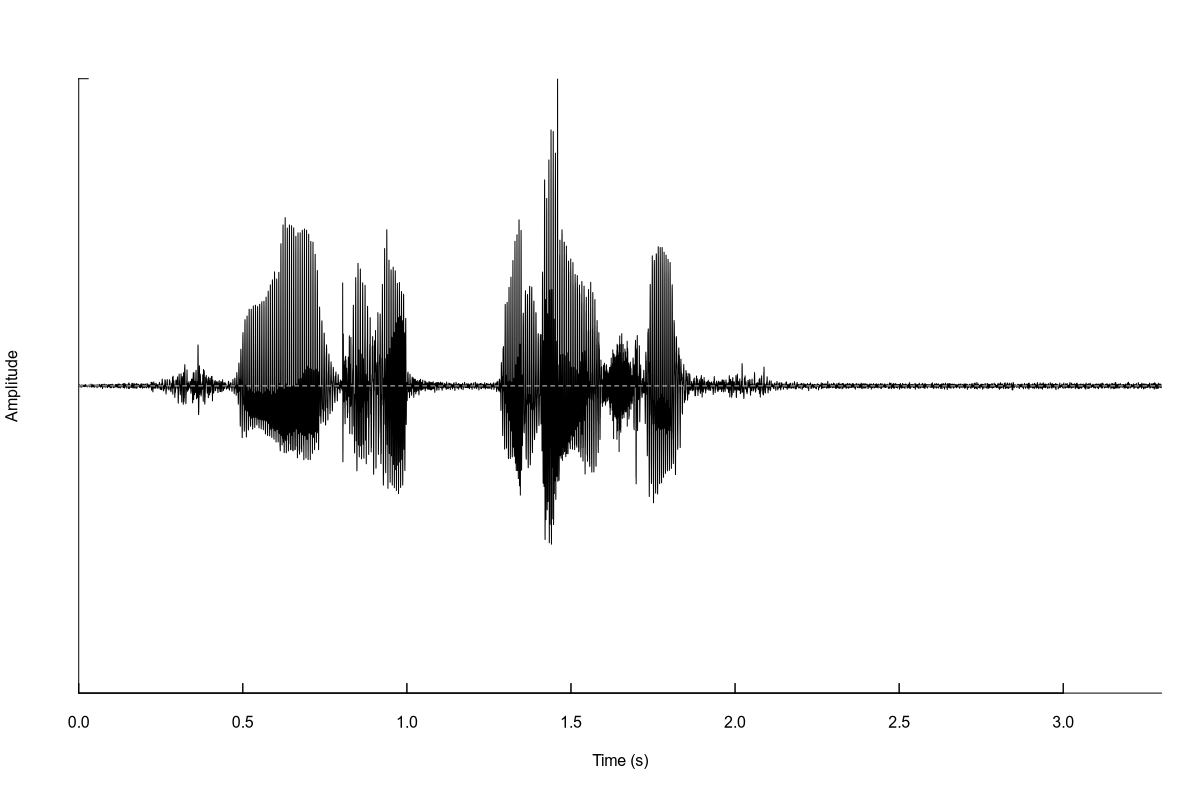
\includegraphics[scale=0.24]{LEVEL_0.png} \\ 
  	Fig.1 Amplitude time graph of low level emotion. \\
  	
  \end{center} 
      \begin{center}
	
	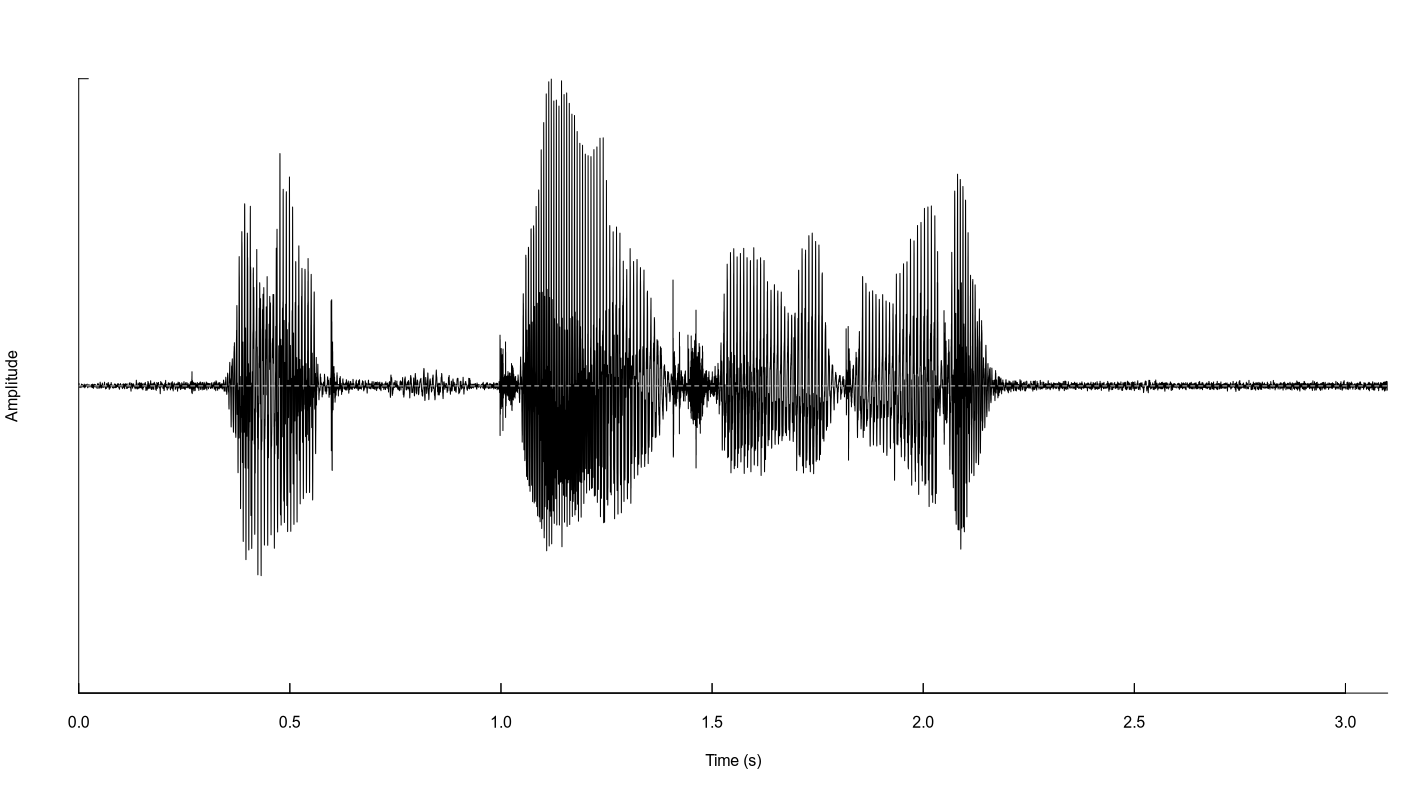
\includegraphics[scale=0.20]{LEVEL_1.png} \\ 
	Fig.2 Amplitude time graph of neutral level emotion. \\
	
\end{center} 
      \begin{center}
	
	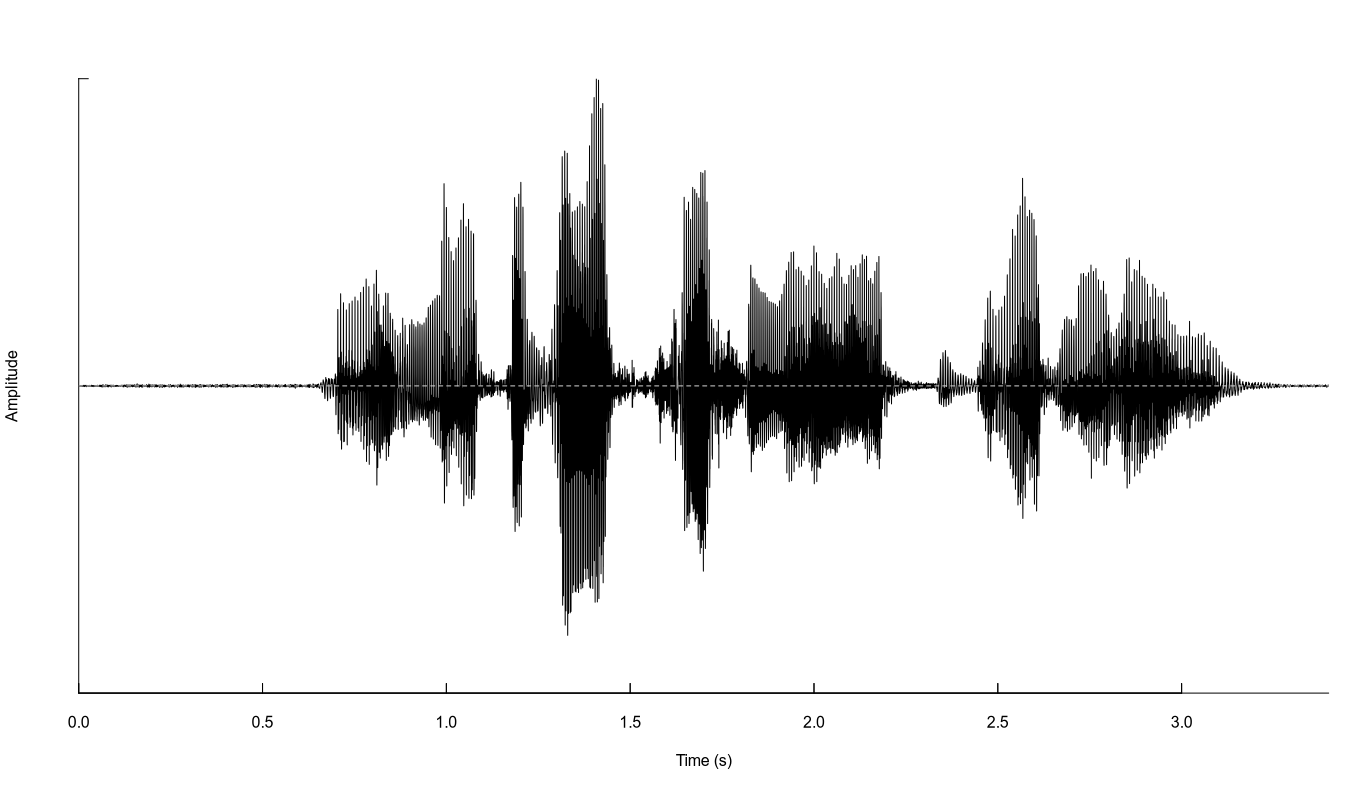
\includegraphics[scale=0.20]{LEVEL_2.png} \\ 
	Fig.3 Amplitude time graph of high level emotion. \\
	
\end{center} 
	\textbf{Frequency}, often known as rate, is a metric that represents how many times an event (n) occurs within a certain time interval (t). The frequency of a sine wave is the number of times an amplitude cycle is repeated in one second. The frequency of a wave on the time axis is known as the conventional frequency or, rather generally, the frequency (f ). Rather of calculating the number of cycles generated every second, it is more common to measure the length of one cycle and then compute the inverse of that length, or the period's reverse (T) \\ 
	\textbf{Zero Crossing Rate} The amount of sign changes c of x(n) per unit of time  (usually one second) is described by the Zero-Crossing Rate (ZCR). A signal with a high ZCR or MCR has a lot of high-frequency material in it. The zero crossing rate of typical harmonic signals is low, and it is proportional to the signal's fundamental frequency. A single pure sine has a zero crossing rate twice its frequency, for example. 
	\subsection{Advanced Audio Features}
	\textbf{\textbf{Mel-Frequency Cepstral Coefficients}}
	Computing Mel-Frequency Cepstral Coefficients is the most common and widely used approach for extracting spectral characteristics (MFCC). MFCCs are one of the most widely used time frequency feature extraction methods in emotion classification techniques like that I am implementing in this project, depending on the Mel scale, which is based on the human ear scale \cite{tsuji2021contact}. Frequency domain characteristics, such as MFCCs, are far more precise than time domain features.\\ Mel-Frequency Cepstral Coefficients (MFCC) are a characterization of a windowed brief signal's actual cepstral produced from the signal's Fast Fourier Transform (FFT). The use of a nonlinear frequency scale, that estimate the behaviour of the auditory cortex, distinguishes it from the true cepstral. Furthermore, these coefficients are accurate and robust in the face of different variants in speakers and recording circumstances. MFCC is an audio feature extraction method that derives parameters from speech that are similar to those utilized by people when hearing speech \cite{paul2021bengali} while de emphasizing all other data. Initially, the voice signal is separated into time frames, each of which contains an arbitrary number of samples. In most applications, frame overlapping is employed to create a seamless transition from one frame to the next. To avoid discontinuities at the edges, every time frame would then be windowed with something like a Hamming window. \\ \\
	$W(n) = 0.54 - 0.46 \cos (\frac{2*\pi*n}{N-1}), 0\le n \le N-1s$ \\ \\
    The numeric variable N represents the total number of sample and n is current sample. Following windowing, the Fast Fourier Transformation (FFT) is used to extract frequency components of a signal in the time domain for each frame.
    For speeding up the whole process, FFT is employed. The Fourier processed frame is passed through the logarithmic Mel-Scaled filter bank. To one 1 kHz, this scale is roughly linear, and at higher frequencies, it becomes logarithmic.\\
    \begin{center}
    
    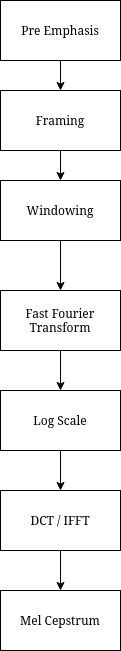
\includegraphics[scale=0.45]{MFCC_PIC.png} \\ 
    Fig.4 The process of Creation of MFCC feature. \\

\end{center} 
The next step is to compute the Discrete Cosine Transformation (DCT) of the filter bank's outputs. The zeroth component is removed since it is untrustworthy, hence DCT ranges coefficients according to relevance. A collection of MFCC  calculated for every speech frame. An acoustical vector is a collection of coefficients that reflects the phonetically relevant aspects of speech and is extremely valuable for any further processing and analyzing in emotion categorization. \\

\begin{minted}[%
	breaklines,
	breakbytoken,
	mathescape,
	linenos,
	numbersep=5pt,
	frame=single,
	numbersep=5pt,
	xleftmargin=0pt,
	]{R}
path = rootPath
num_files = 0
for (i in listFiles){
len = str_length(i)
if(len-2>0) {
format_file = substr(i, len-2, len)
if(format_file == "wav") {
num_files = num_files+1 }}
}
print(num_files)
number_of_cep_features = 20
col_names <- vector(mode = "character",
length = number_of_cep_features)

for (i in 1:number_of_cep_features){
col_names[i]
=
paste("mfcc",as.character(i),sep = "")
}

col_names
[number_of_cep_features+1]="class"
matrix_features = matrix(nrow=num_files,
ncol=number_of_cep_features+1)
colnames(matrix_features)=col_names

for (i in 1:num_files){
audio = readWave(paste(rootPath
,listFiles[i],sep ="/"))
pos = str_locate_all(pattern = "-", 
listFiles[i])
class = substr(listFiles[i],
pos[[1]][4]+1,
pos[[1]][4]+1)
class = as.integer(class)
mfcc = melfcc(audio, sr = audio@samp.rate,
wintime = 0.025,        
hoptime = 0.005,        
numcep = 20,          
sumpower = TRUE,        
nbands = 40,            
bwidth = 1,             
preemph = 0.60,                        
) 
for (j in 1:length(col_names)-1){
matrix_features[i,j]=
mean(mfcc[,j],
na.rm = TRUE)
}
matrix_features
[i,
number_of_cep_features+1]=class
}
	
write.csv( matrix_features, 
"MFCC_FEATURES_EXTRACTED.csv")
	\end{minted}
Code Snippet MFCC Feature Extraction \\ \\
\textbf{Linear Predictive Cepstral Coefficients(LPC)} \\ \\ 
Linear Predictive Coding (LPC) is the most widely used method for simulating human voice output. It works well in clean environments but not very well in chaotic ones. Formant, Short Time Spectrum, Pitch Period, Speech Frame Energy,  bandwidth are the variables for audio signal. LPC is a very essential feature utilised in auditory and speech signal processing that extracts speech properties such as spectra and pitch factors. LPC is also referred as the temporal method since it was created to be equal to the resonant parts of the human vocal cords, which formed the subsequent sound. Each speech sample is first analysed by running it through a filtration system with the purpose of spectrally flattening the signal and making it less susceptible to precision effect \cite{ancilin2021improved}. 
    \begin{center}
	
	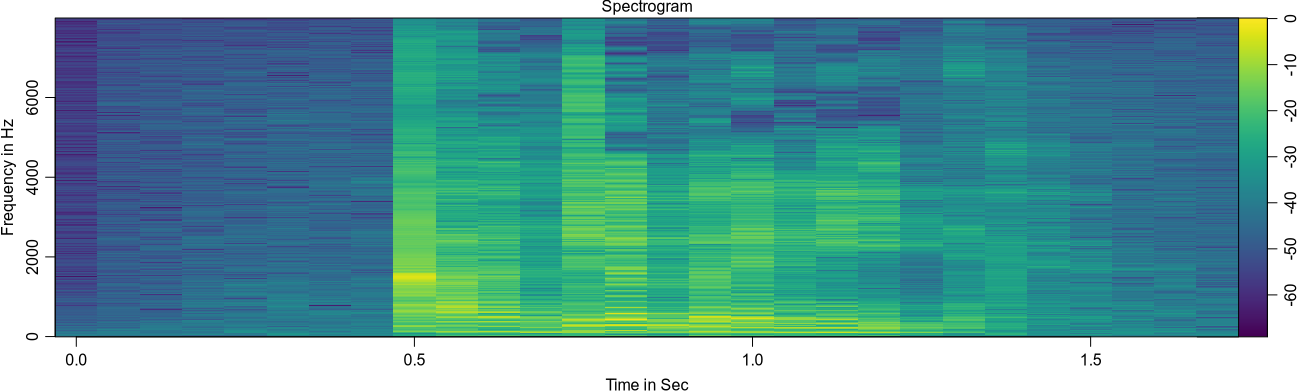
\includegraphics[scale=0.22]{SPECTOGRAM_IMG.png} \\ 
	Fig.5 Spectogram Obtained for finding MFCC features. \\
	
\end{center} 
Filter coefficients should range from 0.9 to 1. Following the pre-emphasis stage, the resultant speech is separated into frames, each of which has M samples lasting 20 to 40 seconds. To assure stillness between frames, there is a customary overlap of 10ms between two consecutive frames. The geometry of the vocal tract determines the nature of the sound produced, according to LPCC. Formant, Pitch Period and Speech Frame Energy are all frequent speech signal components, and LPCC has been one of the most essential methods for estimating them. The objective of feature is to highlight spoken signal using a limited number of signal metrics. We may obtain the LPCC coefficients with the use of LPC, which are then translated into cepstral coefficients. This method works on the principle that one voice sample at any given time can be interpreted as a linear series of previous speech samples \cite{palo2021effect}. Utilizing a first order high filter, the input audio signal is pre emphasised during the first phase, which includes widowing and framing. Because lower frequencies carry greater energy than higher frequencies. Pre emphasis of the resultant signal is done to augment the energy at higher frequencies. 
    \begin{center}
	
	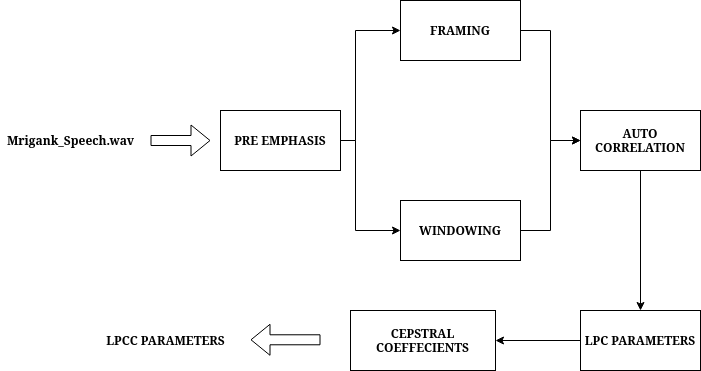
\includegraphics[scale=0.30]{LPCC_PARAMETERS.png} \\ 
	         Fig.6 The process of Creation of LPCC feature. \\
	
\end{center} 

Extracting the audio features of all voice samples in dataset gives us a way to represent each audio in matrix form of features. Using wrassp \cite{wrassp_r} , tuneR  \cite{tune_r}  and signal \cite{singal} packages available in CRAN, audio is read and sampled, then the above mentioned algorithm is applied to get the resultant features of MFCC and LPCC. I use the top 20 features of LPCC and top 20 features of MFCC, this gives us a matrix consisting of rows which represent audio samples and column which represent the audio features. A final class column is added to dataset for the target feature of level of emotion.

    \begin{center}
	
	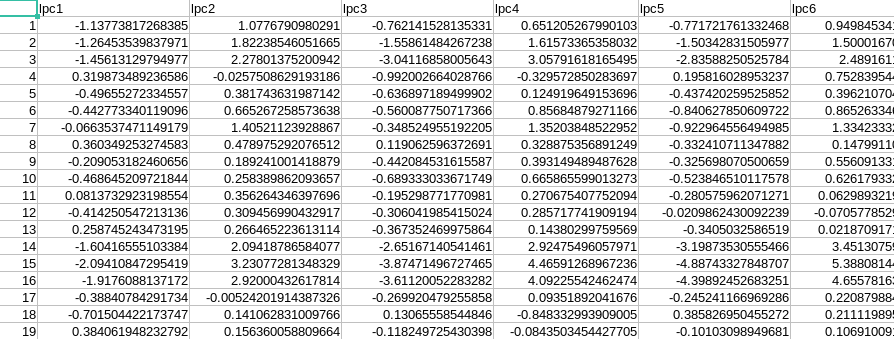
\includegraphics[scale=0.35]{LPC_MFCC_SUBSET_DATASET.png} \\ 
	Fig.7 Subset of final dataset that has all the features. \\
	
\end{center} 

The next step is to use this feature dataset to train various machine learning models, to accurately classify the class of emotion. \\
\textbf{Support Vector Machine}: \\
This is perhaps the most modern methods for supervised machine learning. Support Vector Machine (SVM) models are similar to multilayer perceptron neural networks in that they use support vectors. The concept of a margin on either side of a hyperplane that separate the two data into two classes is important to SVMs.  It has been demonstrated that increasing the margin and therefore generating the biggest possible space between the separating hyperplane and the instances on either side of it reduces the expected generalization error.\\
\textbf{Random Forest}: \\
Random forest is a supervised classification algorithm that is commonly used to solve regression and classification problems. It creates decision trees from various samples, using the simple majority for categorization and the mean for regression. Among the most essential characteristics of the Random Forest Algorithm is that one can accommodate data sets with both categorical and continuous, as in classification and regression problems.
    \begin{center}
	
	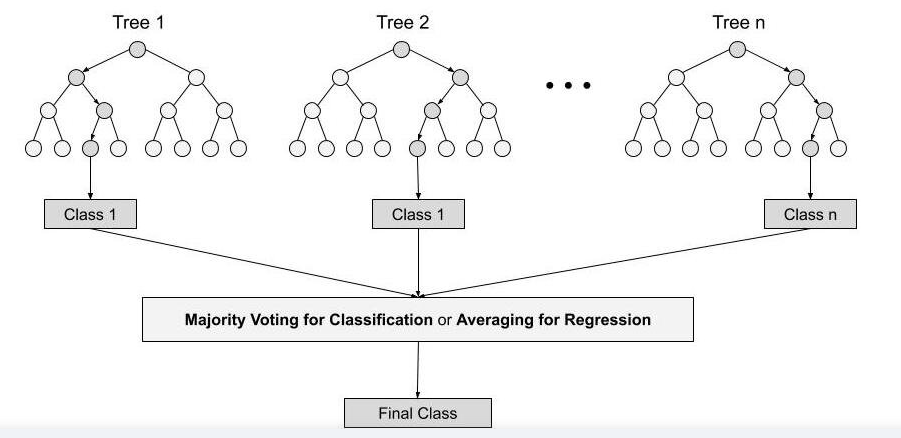
\includegraphics[scale=0.35]{random_forest.png} \\ 
	Fig.8 Random Forest Classification and Regression Algorithm. \cite{random_forest2021} \\
	
\end{center} 
 When it comes to categorization difficulties, it outperforms the competition. In Random Forest, 'M' randomized records are selected at random from a data set with 'K' records. For every sample, a unique decision tree is built. Every decision tree would produce a result \cite{pal2005random}. For regression and classification, the final result is dependent on simple majority or finding the mean of all the results. In this way we can handle both classification problems and in case of variables that are continuous we can also accommodate regression problems. \\ 
 
\textbf{Linear Discriminant Analysis (LDA) }: \\
LDA is a technique used to separate data points by understanding associations among high-dimensional data points as well as the learner vector. It takes high-dimensional data and converts it to linear-dimensional data. It can also be used for data visualisation, categorization, and dimension reduction. Due to its simple structure, the LDA approach frequently yields reliable, good, and understandable classification results. Linear Discriminant Analysis (LDA) is an approach for categorising binary and non-binary features by establishing the connection between the dependent and independent parameters using a linear algorithm \cite{abuzeina2018employing}. It employs the Fischer formula to minimize the data's dimensionality and fit it into a linear dimension. LDA is a classification algorithm, dimensionality reducer, and can also be used as a data visualizer all in one method. The goal of LDA is to reduce inter-class variance by grouping as many comparable data  points as feasible into a single class. There will be reduced misclassifications as a result of this. It also seeks to optimise the distance between the mean of classes, with the mean positioned as far away as feasible to achieve high predictions confidence. 

\section{Results}
 
 \subsection{SVM Radial Kernel}
 The performance of SVM is best with radial kernel as it is able to represent the multidimensional feature of data using radial kernel technique. Although the accuracy of model is not that high. This is due to the fact that most of data points can not be separated that easily by a single maximal margin hyperplane. Hence there is a lot of miss-classifications error in this. The model was able to get a maximum accuracy of 69.98\%.
 \begin{table}[h]
 	\centering
 	\caption{Evaluation metrics of SVM model with Radial Kernel}
 	\begin{tabular}{|l|l|l|l|} 
 		\hline
 		\textbf{Evaluation Metr.} & \textbf{Class:0} & \textbf{Class:1} & \textbf{Class:2}  \\ 
 		\hline
 		Sensitivity                & 0.6027           & 0.7321           & 0.7515            \\ 
 		\hline
 		Specificity                & 0.8783           & 0.8063           & 0.8631            \\ 
 		\hline
 		Pos Pred Value             & 0.6822           & 0.6685           & 0.7471            \\ 
 		\hline
 		Neg Pred Value             & 0.8362           & 0.8495           & 0.8658            \\ 
 		\hline
 		Prevalence                 & 0.3023           & 0.3478           & 0.3499            \\ 
 		\hline
 		Detection Rate             & 0.1822           & 0.2547           & 0.2629            \\ 
 		\hline
 		Detection Preval.       & 0.2671           & 0.3810           & 0.3520            \\ 
 		\hline
 		Balanced Acc.          & 0.7405           & 0.7692           & 0.8073            \\
 		\hline
 	\end{tabular}
 \end{table} 
\begin{table}[h]
	\centering
	\caption{Results of SVM model with Radial Kernel}
	\begin{tabular}{|l|l|} 
		\hline
		\textbf{Metrics}                 & \textbf{Value}    \\ 
		\hline
		Accuracy                         & 0.6998            \\ 
		\hline
		95\% CI                          & (0.6567, 0.7404)  \\ 
		\hline
		No Information Rate              & 0.3499            \\ 
		\hline
		P-Value [Acc \textgreater{} NIR] &  2e-16            \\ 
		\hline
		Kappa                            & 0.5476            \\ 
		\hline
		Mcnemar's Test P-Value           & 0.06448           \\
		\hline
	\end{tabular}
\end{table}
\subsection{Linear Discriminant Analysis}
The performance of LDA is not very good and it perform worst compared to other model that I tried. This is due to the fact that number of features in my datasets are very high. Even a single feature can act as a separating factor for the classes. The approach of transforming all these features into a single line for better separability is not a good idea. As model is not able to capture information of all the feature when it transforms them to a single dimension.
\begin{table} [h]
	\centering
	\caption{Evaluation metrics of Linear Discriminant Analysis model.}
	\begin{tabular}{|l|l|l|l|} 
		\hline
		\textbf{Evaluation Metr.} & \textbf{Class:0} & \textbf{Class:1} & \textbf{Class:2}  \\ 
		\hline
		Sensitivity                 & 0.5137           & 0.6429           & 0.4852            \\ 
		\hline
		Specificity                 & 0.8338           & 0.6540           & 0.8312            \\ 
		\hline
		Pos Pred Value              & 0.5725           & 0.4977           & 0.6074            \\ 
		\hline
		Neg Pred Value              & 0.7983           & 0.7744           & 0.7500            \\ 
		\hline
		Prevalence                  & 0.3023           & 0.3478           & 0.3499            \\ 
		\hline
		Detection Rate              & 0.1553           & 0.2236           & 0.1698            \\ 
		\hline
		Detection Prev.      & 0.2712           & 0.4493           & 0.2795            \\ 
		\hline
		Balanced Acc.        & 0.6738           & 0.6484           & 0.6582            \\
		\hline
	\end{tabular}
\end{table}
\begin{table}[h]
	\centering
	\caption{Results of Linear Discriminant Analysis model.}
	\begin{tabular}{|l|l|} 
		\hline
		\textbf{Metrics}                 & \textbf{Value}    \\ 
		\hline
		Accuracy                         & 0.5487            \\ 
		\hline
		95\% CI                          & (0.5031, 0.5937)  \\ 
		\hline
		No Information Rate              & 0.3499            \\ 
		\hline
		P-Value [Acc \textgreater{} NIR] &  2.2e-16          \\ 
		\hline
		Kappa                            & 0.3202            \\ 
		\hline
		Mcnemar's Test P-Value           & 0.001641          \\
		\hline
	\end{tabular}
\end{table}
\subsection{Random Forest}
Random forest performs the best among all the models. The model is able to get an accuracy of 100\%. The reason for its good performance is rule based approach that is able to select the best feature which provide the highest information gain at each node split. As it is an ensemble model as well, we are able to use many decision trees that use different subset of features for building. Then when majority algorithm is applied for final class value selection, it is able to provide highly accurate results.
\begin{table}[h]
	\centering
	\caption{Evaluation metrics of Random Forest model.}
	\begin{tabular}{|l|l|l|l|} 
		\hline
		\textbf{Evaluation Met.} & \textbf{Class:0} & \textbf{Class:1} & \textbf{Class:2} \\ 
		\hline
		Sensitivity                 & 1.000          & 1.000           & 1.000           \\ 
		\hline
		Specificity                 & 1.000           & 1.000           & 1.000           \\ 
		\hline
		Pos Pred Value              & 1.000           & 1.000           & 1.000           \\ 
		\hline
		Neg Pred Value              & 1.000           & 1.000           & 1.000           \\ 
		\hline
		Prevalence                  & 0.302           & 0.348         & 0.349        \\ 
		\hline
		Detection Rate              & 0.302     & 0.348           & 0.349           \\ 
		\hline
		Detection Preval.       & 0.302        & 0.348           & 0.349           \\ 
		\hline
		Balanced Acc.      & 1.000           & 1.000           & 1.000           \\
		\hline
	\end{tabular}
\end{table}
\begin{table}[h]
	\centering
	\caption{Results of Random Forest model.}
	\begin{tabular}{|l|l|} 
		\hline
		\textbf{Metrics}                 & \textbf{Value}  \\ 
		\hline
		Accuracy                         & 1               \\ 
		\hline
		95\% CI                          & (0.9924, 1)     \\ 
		\hline
		No Information Rate              & 0.3499          \\ 
		\hline
		P-Value [Acc \textgreater{} NIR] &  2.2e-16        \\ 
		\hline
		Kappa                            & 1               \\ 
		\hline
		Mcnemar's Test P-Value           & NA              \\
		\hline
	\end{tabular}
\end{table}
A sample image of the model when it is deployed using R Shiny is provided below. The used can upload the audio samples using the GUI provided, the app will then print the emotion of the audio samples.
    \begin{center}
	
	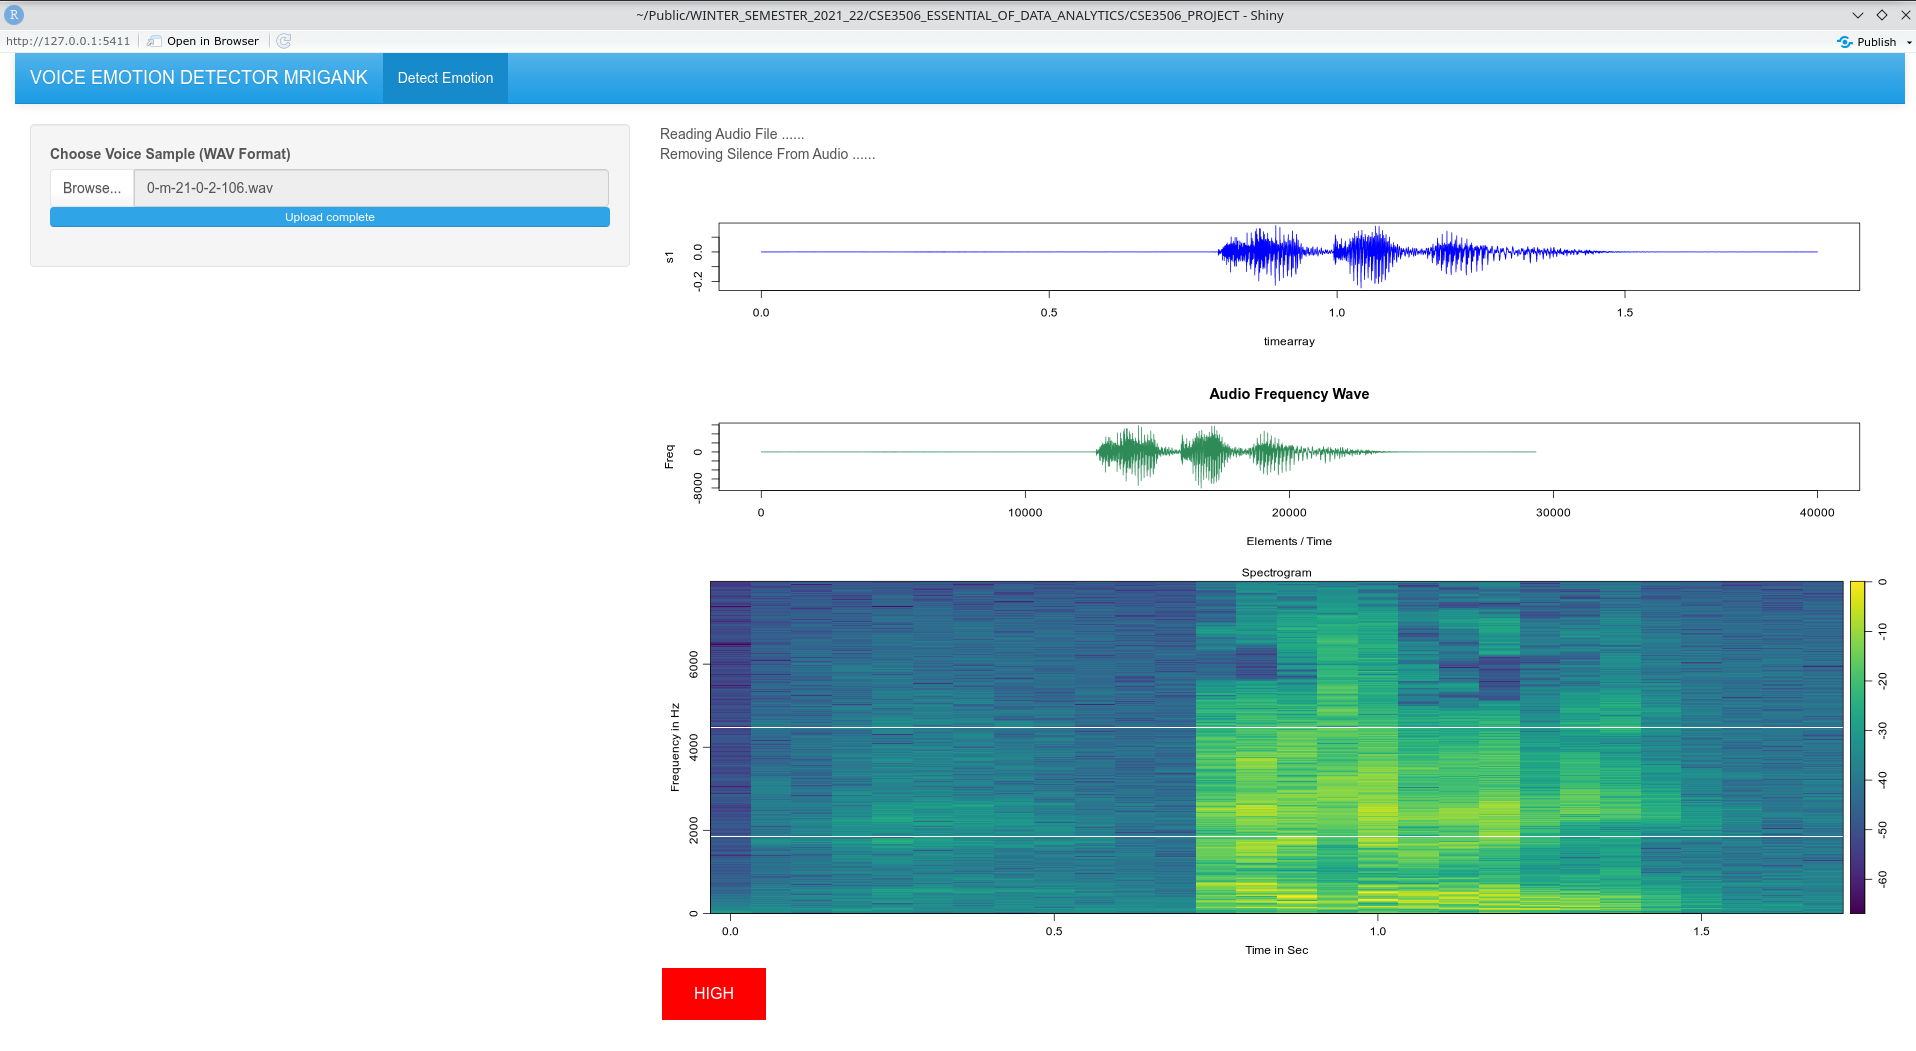
\includegraphics[scale=0.15]{deployment_CSE3506_pic.png} \\ 
	Fig 9 Emotion Classification app deployed on R Shiny.\\
	
\end{center} 

\section{Conclusion and Future Work}
I was able to get an accuracy of 100\% using random forest model, which is very good when compared with existing models for BAVED dataset. The immense potential of machine learning and deep learning can take emotion classification to a new level. I have used only a single language and the audio samples are not super long. A similar model can be applied for large audio files, or continuous audio streaming, where each chunk of audio can be labeled as a one emotion type. We can also gather a larger dataset which has a noisy recordings as well, so that we can deploy this model in real time systems as well. Audio samples from different languages can also be utilized which will make this model truly robust and global in approach.
	\bibliographystyle{acl_natbib}
	\bibliography{anthology,acl2021}
	
	%\appendix
	
	
	
\end{document}
